\documentclass[12pt,a4paper]{article}
\usepackage[utf8]{vietnam}
\usepackage{amsmath,amssymb}
\usepackage{tabularx}
\usepackage{tikz}
\usepackage{xcolor}
\usepackage[top=0.6cm, bottom=0.6cm, left=0.6cm, right=0.6cm]{geometry}
\usepackage[dethi]{ex_test}

\SAOPTN{widthSA=2.6,heightSA=0.62}

\setlength{\parskip}{0pt}

% Dòng kẻ chấm mờ đều đặn chuẩn viết tay
\newcommand{\dongke}[1]{%
  \begingroup%
  \setlength{\parskip}{0pt}%
  \baselineskip=18.5pt%
  \vspace{1.0mm}%
  \foreach \i in {1,...,#1}{%
    \noindent{\color{gray!60}\dotfill}\par%
  }%
  \vspace{0.6mm}%
  \endgroup%
}

% Định nghĩa ô bài tập tự luận trong bảng
\newcommand{\oBaiTap}[3][6]{%
  \vspace{1.0mm}%
  \noindent\textbf{#2} #3\par%
  \dongke{#1}%
}

\begin{document}
\pagestyle{empty}
% =============================================================================
% ========================= TOÁN 7 - TUẦN 07 - BUỔI 02: MÃ ĐỀ 101 =============
% ========================= MẶT TRƯỚC (TRANG 1/2) ==============================
% =============================================================================

\noindent
\begin{tabularx}{\linewidth}{|X|c|}
\hline
\textbf{PHIẾU KIỂM TRA ĐỊNH KỲ TOÁN 7 - TUẦN 07 - BUỔI 02} & \textbf{Mã đề: 101 - Trang 1/2} \\
\hline
\end{tabularx}

\vspace{1.2mm}

\noindent
\begin{tabularx}{\linewidth}{|p{3.2cm}|X|}
\hline
\centering\textbf{ĐIỂM SỐ} & \centering\textbf{LỜI NHẬN XÉT CỦA THẦY CÔ} \tabularnewline
\hline
\rule{0pt}{1.8cm} & \tabularnewline
\hline
\end{tabularx}

\vspace{1.5mm}

\noindent\textbf{Câu 1 (0,25 điểm).} Số đối của số hữu tỉ $-\frac{7}{12}$ bằng bao nhiêu? \shortans{\frac{7}{12}}\par\vspace{0.5mm}
\noindent\textbf{Câu 2 (0,25 điểm).} Giá trị của biểu thức $\left(-\frac{2}{3}\right)^3$ bằng bao nhiêu? \shortans{-\frac{8}{27}}\par\vspace{0.5mm}
\noindent\textbf{Câu 3 (0,25 điểm).} Giá trị của căn bậc hai số học $\sqrt{\frac{49}{81}}$ bằng bao nhiêu? \shortans{\frac{7}{9}}\par\vspace{0.5mm}
\noindent\textbf{Câu 4 (0,25 điểm).} Tính giá trị của biểu thức $\lvert -7{,}5\rvert + \lvert -2{,}5\rvert$. \shortans{10}\par\vspace{0.5mm}
\noindent\textbf{Câu 5 (0,25 điểm).} Làm tròn số $15{,}374$ đến hàng phần trăm được kết quả là: \shortans{15{,}37}\par\vspace{0.5mm}
\noindent\textbf{Câu 6 (0,25 điểm).} Cho hai góc $\widehat{aOb}$ và $\widehat{bOc}$ kề bù, biết $\widehat{aOb}=65^\circ$. Số đo góc $\widehat{bOc}$ là: \shortans{115^\circ}\par\vspace{0.5mm}
\noindent\textbf{Câu 7 (0,25 điểm).} Tia $Oz$ là phân giác của góc $\widehat{xOy}$. Biết $\widehat{xOz}=40^\circ$, số đo $\widehat{xOy}$ là: \shortans{80^\circ}\par\vspace{0.5mm}
\noindent\textbf{Câu 8 (0,25 điểm).} Một định lí gồm hai phần là Kết luận và phần nào? \shortans{\text{Giả thiết}}\par\vspace{0.5mm}
\noindent\textbf{Câu 9 (0,25 điểm).} Cho $a \perp c$ và $b \perp c$ ($a \ne b$). Quan hệ giữa hai đường thẳng $a$ và $b$ là: \shortans{\text{song song}}\par\vspace{0.5mm}
\noindent\textbf{Câu 10 (0,25 điểm).} Hộp bút giá $50\,000$ đ, giảm giá $20\%$. Số tiền người mua phải trả là: \shortans{40\,000\text{ đ}}\par\vspace{0.5mm}
\vspace{0.6mm}

\noindent\textbf{Câu 11 (2,0 điểm). Thực hiện phép tính (hợp lý nếu có thể):}
\vspace{0.8mm}

\noindent
\begin{tabularx}{\linewidth}{|X|X|}
\hline
\oBaiTap[10]{a)}{$\frac{7}{12} + \left(-\frac{5}{6}\right) + \frac{5}{12}$} & 
\oBaiTap[10]{b)}{$\frac{13}{17} \cdot \left(-\frac{5}{9}\right) + \frac{13}{17} \cdot \left(-\frac{4}{9}\right)$} \\
\hline
\oBaiTap[10]{c)}{$\left(-\frac{1}{2}\right)^3 \cdot 8 - 1{,}25 \cdot 4$} & 
\oBaiTap[10]{d)}{$\sqrt{\frac{49}{16}} - \lvert -0{,}75\rvert + \sqrt{64}$} \\
\hline
\end{tabularx}

\newpage
% =============================================================================
% ========================= TOÁN 7 - TUẦN 07 - BUỔI 02: MÃ ĐỀ 101 =============
% ========================= MẶT SAU (TRANG 2/2) ================================
% =============================================================================

\noindent
\begin{tabularx}{\linewidth}{|X|c|}
\hline
\textbf{TOÁN 7 - TUẦN 07 - BUỔI 02} & \textbf{Mã đề: 101 - Trang 2/2} \\
\hline
\end{tabularx}

\vspace{1.2mm}

\noindent\textbf{Câu 12 (2,0 điểm). Tìm số hữu tỉ $x$, biết:}
\vspace{0.6mm}

\noindent
\begin{tabularx}{\linewidth}{|X|X|}
\hline
\oBaiTap[5]{a)}{$x + \frac{1}{3} = \frac{5}{6}$} & 
\oBaiTap[5]{b)}{$\frac{2}{3}x - \frac{1}{2} = \frac{5}{6}$} \\
\hline
\oBaiTap[5]{c)}{$\left(x - \frac{1}{2}\right)^2 = \frac{9}{16}$} & 
\oBaiTap[5]{d)}{$\lvert 2x - 1\rvert = 5$} \\
\hline
\end{tabularx}

\vspace{1.2mm}

\noindent
\begin{tabularx}{\linewidth}{|X|}
\hline
\vspace{0.5mm}
\begin{minipage}[t]{0.65\linewidth}
\vspace{0pt}
\textbf{Câu 13 (2,5 điểm).} Cho hình vẽ bên, biết hai đường thẳng $a$ và $b$ cùng vuông góc với đường thẳng $AB$ lần lượt tại $A$ và $B$. Đường thẳng $c$ cắt $a$ tại $C$ và cắt $b$ tại $D$ sao cho $\widehat{ACD} = 70^\circ$.\par\vspace{0.4mm}
\textbf{a) (1,25 điểm)} Chứng minh rằng đường thẳng $a$ song song với đường thẳng $b$ ($a \parallel b$).\par\vspace{0.4mm}
\textbf{b) (1,25 điểm)} Tính số đo góc $\widehat{BDC}$ và góc $\widehat{D}_1$.
\end{minipage}\hfill
\begin{minipage}[t]{0.33\linewidth}
\vspace{0pt}\centering
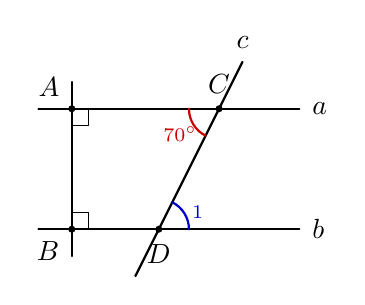
\begin{tikzpicture}[scale=0.85, >=stealth, line join=round, line cap=round]
  % Duong thang vuong goc AB
  \draw[thick] (0.8, 0.3) -- (0.8, 2.9);
  % Duong thang a di qua A
  \draw[thick] (0.3, 2.5) -- (4.2, 2.5) node[right=1pt] {$a$};
  % Duong thang b di qua B
  \draw[thick] (0.3, 0.7) -- (4.2, 0.7) node[right=1pt] {$b$};
  % Cat tuyen c di qua C va D (C(3.0, 2.5) va D(2.1, 0.7))
  \draw[thick] (3.35, 3.2) node[above=1pt] {$c$} -- (1.75, -0.0);
  
  % Giao diem A va B
  \fill (0.8, 2.5) circle (1.5pt) node[above left=1pt] {$A$};
  \fill (0.8, 0.7) circle (1.5pt) node[below left=1pt] {$B$};
  % Ky hieu vuong goc tai A va B
  \draw (0.8, 2.25) -- (1.05, 2.25) -- (1.05, 2.5);
  \draw (0.8, 0.95) -- (1.05, 0.95) -- (1.05, 0.7);
  
  % Giao diem C va D
  \fill (3.0, 2.5) circle (1.5pt) node[above=2pt] {$C$};
  \fill (2.1, 0.7) circle (1.5pt) node[below=2pt] {$D$};
  
  % Cung goc nhon ACD (huong tu 180 do ve 243.4 do)
  \draw[red!80!black, thick] (3.0, 2.5) ++(180:0.45) arc (180:243.4:0.45);
  \node[red!80!black, font=\scriptsize] at (2.42, 2.12) {$70^\circ$};
  
  % Cung goc D1 (so le trong voi ACD)
  \draw[blue!80!black, thick] (2.1, 0.7) ++(0:0.45) arc (0:63.4:0.45);
  \node[blue!80!black, font=\scriptsize] at (2.68, 0.95) {$1$};
\end{tikzpicture}
\end{minipage}\par
\vspace{0.5mm}
\noindent\textit{Bài giải:}\dongke{9}
\\ \hline
\end{tabularx}

\vspace{1.2mm}

\noindent
\begin{tabularx}{\linewidth}{|X|}
\hline
\vspace{0.5mm}
\begin{minipage}[t]{0.65\linewidth}
\vspace{0pt}
\textbf{Câu 14 (1,0 điểm).} Cho hình vẽ bên, biết hai đường thẳng $x$ và $y$ cùng vuông góc với đường thẳng $MN$ lần lượt tại $M$ và $N$. Đường thẳng $d$ cắt $x$ tại $P$ và cắt $y$ tại $Q$ sao cho $\widehat{MPQ} = 60^\circ$.\par\vspace{0.4mm}
\textbf{a) (0,5 điểm)} Chứng minh rằng đường thẳng $x$ song song với đường thẳng $y$ ($x \parallel y$).\par\vspace{0.4mm}
\textbf{b) (0,5 điểm)} Tính số đo góc $\widehat{NQP}$ và góc $\widehat{Q}_1$.
\end{minipage}\hfill
\begin{minipage}[t]{0.33\linewidth}
\vspace{0pt}\centering
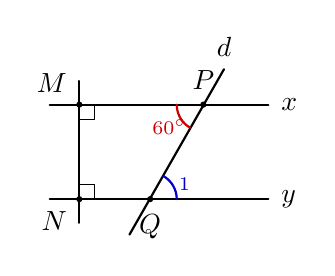
\begin{tikzpicture}[scale=0.75, >=stealth, line join=round, line cap=round]
  % Duong thang vuong goc MN
  \draw[thick] (0.8, 0.2) -- (0.8, 2.6);
  % Duong thang x di qua M
  \draw[thick] (0.3, 2.2) -- (4.0, 2.2) node[right=1pt] {$x$};
  % Duong thang y di qua N
  \draw[thick] (0.3, 0.6) -- (4.0, 0.6) node[right=1pt] {$y$};
  % Cat tuyen d di qua P va Q
  \draw[thick] (3.25, 2.8) node[above=1pt] {$d$} -- (1.65, -0.0);
  
  % Giao diem M va N
  \fill (0.8, 2.2) circle (1.5pt) node[above left=1pt] {$M$};
  \fill (0.8, 0.6) circle (1.5pt) node[below left=1pt] {$N$};
  % Ky hieu vuong goc tai M va N
  \draw (0.8, 1.95) -- (1.05, 1.95) -- (1.05, 2.2);
  \draw (0.8, 0.85) -- (1.05, 0.85) -- (1.05, 0.6);
  
  % Giao diem P va Q
  \fill (2.9, 2.2) circle (1.5pt) node[above=2pt] {$P$};
  \fill (2.0, 0.6) circle (1.5pt) node[below=2pt] {$Q$};
  
  % Cung goc nhon MPQ
  \draw[red!80!black, thick] (2.9, 2.2) ++(180:0.45) arc (180:240.6:0.45);
  \node[red!80!black, font=\scriptsize] at (2.32, 1.82) {$60^\circ$};
  
  % Cung goc Q1 (so le trong voi MPQ)
  \draw[blue!80!black, thick] (2.0, 0.6) ++(0:0.45) arc (0:60.6:0.45);
  \node[blue!80!black, font=\scriptsize] at (2.58, 0.85) {$1$};
\end{tikzpicture}
\end{minipage}\par
\vspace{0.4mm}
\noindent\textit{Bài giải:}\dongke{6}
\\ \hline
\end{tabularx}

\newpage

% =============================================================================
% ========================= TOÁN 7 - TUẦN 07 - BUỔI 02: MÃ ĐỀ 102 =============
% ========================= MẶT TRƯỚC (TRANG 1/2) ==============================
% =============================================================================

\noindent
\begin{tabularx}{\linewidth}{|X|c|}
\hline
\textbf{PHIẾU KIỂM TRA ĐỊNH KỲ TOÁN 7 - TUẦN 07 - BUỔI 02} & \textbf{Mã đề: 102 - Trang 1/2} \\
\hline
\end{tabularx}

\vspace{1.2mm}

\noindent
\begin{tabularx}{\linewidth}{|p{3.2cm}|X|}
\hline
\centering\textbf{ĐIỂM SỐ} & \centering\textbf{LỜI NHẬN XÉT CỦA THẦY CÔ} \tabularnewline
\hline
\rule{0pt}{1.8cm} & \tabularnewline
\hline
\end{tabularx}

\vspace{1.5mm}

\noindent\textbf{Câu 1 (0,25 điểm).} Số đối của số hữu tỉ $-\frac{9}{14}$ bằng bao nhiêu? \shortans{\frac{9}{14}}\par\vspace{0.5mm}
\noindent\textbf{Câu 2 (0,25 điểm).} Giá trị của biểu thức $\left(-\frac{3}{2}\right)^3$ bằng bao nhiêu? \shortans{-\frac{27}{8}}\par\vspace{0.5mm}
\noindent\textbf{Câu 3 (0,25 điểm).} Giá trị của căn bậc hai số học $\sqrt{\frac{64}{121}}$ bằng bao nhiêu? \shortans{\frac{8}{11}}\par\vspace{0.5mm}
\noindent\textbf{Câu 4 (0,25 điểm).} Tính giá trị của biểu thức $\lvert -8{,}4\rvert + \lvert -1{,}6\rvert$. \shortans{10}\par\vspace{0.5mm}
\noindent\textbf{Câu 5 (0,25 điểm).} Làm tròn số $24{,}682$ đến hàng phần trăm được kết quả là: \shortans{24{,}68}\par\vspace{0.5mm}
\noindent\textbf{Câu 6 (0,25 điểm).} Cho hai góc $\widehat{aOb}$ và $\widehat{bOc}$ kề bù, biết $\widehat{aOb}=45^\circ$. Số đo góc $\widehat{bOc}$ là: \shortans{135^\circ}\par\vspace{0.5mm}
\noindent\textbf{Câu 7 (0,25 điểm).} Tia $Oz$ là phân giác của góc $\widehat{xOy}$. Biết $\widehat{xOz}=35^\circ$, số đo $\widehat{xOy}$ là: \shortans{70^\circ}\par\vspace{0.5mm}
\noindent\textbf{Câu 8 (0,25 điểm).} Trong định lí dạng ''Nếu $P$ thì $Q$'', phần $P$ được gọi là gì? \shortans{\text{Giả thiết}}\par\vspace{0.5mm}
\noindent\textbf{Câu 9 (0,25 điểm).} Cho $a \parallel b$. Nếu đường thẳng $c \perp a$ thì đường thẳng $c$ có quan hệ gì với $b$? \shortans{\text{vuông góc}}\par\vspace{0.5mm}
\noindent\textbf{Câu 10 (0,25 điểm).} Chiếc compa giá $40\,000$ đ, giảm giá $20\%$. Số tiền người mua phải trả là: \shortans{32\,000\text{ đ}}\par\vspace{0.5mm}
\vspace{0.6mm}

\noindent\textbf{Câu 11 (2,0 điểm). Thực hiện phép tính (hợp lý nếu có thể):}
\vspace{0.8mm}

\noindent
\begin{tabularx}{\linewidth}{|X|X|}
\hline
\oBaiTap[10]{a)}{$\frac{8}{15} + \left(-\frac{3}{4}\right) + \frac{7}{15}$} & 
\oBaiTap[10]{b)}{$\frac{15}{19} \cdot \left(-\frac{7}{11}\right) + \frac{15}{19} \cdot \left(-\frac{4}{11}\right)$} \\
\hline
\oBaiTap[10]{c)}{$\left(-\frac{1}{3}\right)^2 \cdot 27 - 2{,}5 \cdot 2$} & 
\oBaiTap[10]{d)}{$\sqrt{\frac{81}{25}} - \lvert -0{,}8\rvert + \sqrt{49}$} \\
\hline
\end{tabularx}

\newpage
% =============================================================================
% ========================= TOÁN 7 - TUẦN 07 - BUỔI 02: MÃ ĐỀ 102 =============
% ========================= MẶT SAU (TRANG 2/2) ================================
% =============================================================================

\noindent
\begin{tabularx}{\linewidth}{|X|c|}
\hline
\textbf{TOÁN 7 - TUẦN 07 - BUỔI 02} & \textbf{Mã đề: 102 - Trang 2/2} \\
\hline
\end{tabularx}

\vspace{1.2mm}

\noindent\textbf{Câu 12 (2,0 điểm). Tìm số hữu tỉ $x$, biết:}
\vspace{0.6mm}

\noindent
\begin{tabularx}{\linewidth}{|X|X|}
\hline
\oBaiTap[5]{a)}{$x + \frac{1}{4} = \frac{7}{8}$} & 
\oBaiTap[5]{b)}{$\frac{3}{4}x - \frac{1}{3} = \frac{5}{12}$} \\
\hline
\oBaiTap[5]{c)}{$\left(x + \frac{1}{3}\right)^2 = \frac{25}{9}$} & 
\oBaiTap[5]{d)}{$\lvert 2x + 1\rvert = 7$} \\
\hline
\end{tabularx}

\vspace{1.2mm}

\noindent
\begin{tabularx}{\linewidth}{|X|}
\hline
\vspace{0.5mm}
\begin{minipage}[t]{0.65\linewidth}
\vspace{0pt}
\textbf{Câu 13 (2,5 điểm).} Cho hình vẽ bên, biết hai đường thẳng $a$ và $b$ cùng vuông góc với đường thẳng $AB$ lần lượt tại $A$ và $B$. Đường thẳng $c$ cắt $a$ tại $C$ và cắt $b$ tại $D$ sao cho $\widehat{ACD} = 65^\circ$.\par\vspace{0.4mm}
\textbf{a) (1,25 điểm)} Chứng minh rằng đường thẳng $a$ song song với đường thẳng $b$ ($a \parallel b$).\par\vspace{0.4mm}
\textbf{b) (1,25 điểm)} Tính số đo góc $\widehat{BDC}$ và góc $\widehat{D}_1$.
\end{minipage}\hfill
\begin{minipage}[t]{0.33\linewidth}
\vspace{0pt}\centering
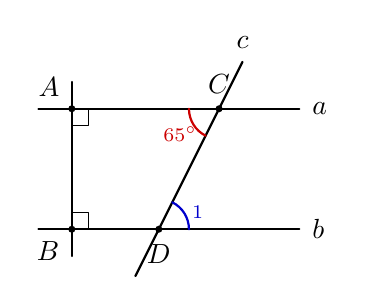
\begin{tikzpicture}[scale=0.85, >=stealth, line join=round, line cap=round]
  % Duong thang vuong goc AB
  \draw[thick] (0.8, 0.3) -- (0.8, 2.9);
  % Duong thang a di qua A
  \draw[thick] (0.3, 2.5) -- (4.2, 2.5) node[right=1pt] {$a$};
  % Duong thang b di qua B
  \draw[thick] (0.3, 0.7) -- (4.2, 0.7) node[right=1pt] {$b$};
  % Cat tuyen c di qua C va D (C(3.0, 2.5) va D(2.1, 0.7))
  \draw[thick] (3.35, 3.2) node[above=1pt] {$c$} -- (1.75, -0.0);
  
  % Giao diem A va B
  \fill (0.8, 2.5) circle (1.5pt) node[above left=1pt] {$A$};
  \fill (0.8, 0.7) circle (1.5pt) node[below left=1pt] {$B$};
  % Ky hieu vuong goc tai A va B
  \draw (0.8, 2.25) -- (1.05, 2.25) -- (1.05, 2.5);
  \draw (0.8, 0.95) -- (1.05, 0.95) -- (1.05, 0.7);
  
  % Giao diem C va D
  \fill (3.0, 2.5) circle (1.5pt) node[above=2pt] {$C$};
  \fill (2.1, 0.7) circle (1.5pt) node[below=2pt] {$D$};
  
  % Cung goc nhon ACD (huong tu 180 do ve 243.4 do)
  \draw[red!80!black, thick] (3.0, 2.5) ++(180:0.45) arc (180:243.4:0.45);
  \node[red!80!black, font=\scriptsize] at (2.42, 2.12) {$65^\circ$};
  
  % Cung goc D1 (so le trong voi ACD)
  \draw[blue!80!black, thick] (2.1, 0.7) ++(0:0.45) arc (0:63.4:0.45);
  \node[blue!80!black, font=\scriptsize] at (2.68, 0.95) {$1$};
\end{tikzpicture}
\end{minipage}\par
\vspace{0.5mm}
\noindent\textit{Bài giải:}\dongke{9}
\\ \hline
\end{tabularx}

\vspace{1.2mm}

\noindent
\begin{tabularx}{\linewidth}{|X|}
\hline
\vspace{0.5mm}
\begin{minipage}[t]{0.65\linewidth}
\vspace{0pt}
\textbf{Câu 14 (1,0 điểm).} Cho hình vẽ bên, biết hai đường thẳng $x$ và $y$ cùng vuông góc với đường thẳng $MN$ lần lượt tại $M$ và $N$. Đường thẳng $d$ cắt $x$ tại $P$ và cắt $y$ tại $Q$ sao cho $\widehat{MPQ} = 55^\circ$.\par\vspace{0.4mm}
\textbf{a) (0,5 điểm)} Chứng minh rằng đường thẳng $x$ song song với đường thẳng $y$ ($x \parallel y$).\par\vspace{0.4mm}
\textbf{b) (0,5 điểm)} Tính số đo góc $\widehat{NQP}$ và góc $\widehat{Q}_1$.
\end{minipage}\hfill
\begin{minipage}[t]{0.33\linewidth}
\vspace{0pt}\centering
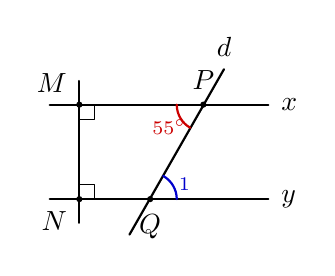
\begin{tikzpicture}[scale=0.75, >=stealth, line join=round, line cap=round]
  % Duong thang vuong goc MN
  \draw[thick] (0.8, 0.2) -- (0.8, 2.6);
  % Duong thang x di qua M
  \draw[thick] (0.3, 2.2) -- (4.0, 2.2) node[right=1pt] {$x$};
  % Duong thang y di qua N
  \draw[thick] (0.3, 0.6) -- (4.0, 0.6) node[right=1pt] {$y$};
  % Cat tuyen d di qua P va Q
  \draw[thick] (3.25, 2.8) node[above=1pt] {$d$} -- (1.65, -0.0);
  
  % Giao diem M va N
  \fill (0.8, 2.2) circle (1.5pt) node[above left=1pt] {$M$};
  \fill (0.8, 0.6) circle (1.5pt) node[below left=1pt] {$N$};
  % Ky hieu vuong goc tai M va N
  \draw (0.8, 1.95) -- (1.05, 1.95) -- (1.05, 2.2);
  \draw (0.8, 0.85) -- (1.05, 0.85) -- (1.05, 0.6);
  
  % Giao diem P va Q
  \fill (2.9, 2.2) circle (1.5pt) node[above=2pt] {$P$};
  \fill (2.0, 0.6) circle (1.5pt) node[below=2pt] {$Q$};
  
  % Cung goc nhon MPQ
  \draw[red!80!black, thick] (2.9, 2.2) ++(180:0.45) arc (180:240.6:0.45);
  \node[red!80!black, font=\scriptsize] at (2.32, 1.82) {$55^\circ$};
  
  % Cung goc Q1 (so le trong voi MPQ)
  \draw[blue!80!black, thick] (2.0, 0.6) ++(0:0.45) arc (0:60.6:0.45);
  \node[blue!80!black, font=\scriptsize] at (2.58, 0.85) {$1$};
\end{tikzpicture}
\end{minipage}\par
\vspace{0.4mm}
\noindent\textit{Bài giải:}\dongke{6}
\\ \hline
\end{tabularx}

\newpage

% =============================================================================
% ========================= TOÁN 7 - TUẦN 07 - BUỔI 02: MÃ ĐỀ 103 =============
% ========================= MẶT TRƯỚC (TRANG 1/2) ==============================
% =============================================================================

\noindent
\begin{tabularx}{\linewidth}{|X|c|}
\hline
\textbf{PHIẾU KIỂM TRA ĐỊNH KỲ TOÁN 7 - TUẦN 07 - BUỔI 02} & \textbf{Mã đề: 103 - Trang 1/2} \\
\hline
\end{tabularx}

\vspace{1.2mm}

\noindent
\begin{tabularx}{\linewidth}{|p{3.2cm}|X|}
\hline
\centering\textbf{ĐIỂM SỐ} & \centering\textbf{LỜI NHẬN XÉT CỦA THẦY CÔ} \tabularnewline
\hline
\rule{0pt}{1.8cm} & \tabularnewline
\hline
\end{tabularx}

\vspace{1.5mm}

\noindent\textbf{Câu 1 (0,25 điểm).} Số đối của số hữu tỉ $-\frac{8}{15}$ bằng bao nhiêu? \shortans{\frac{8}{15}}\par\vspace{0.5mm}
\noindent\textbf{Câu 2 (0,25 điểm).} Giá trị của biểu thức $\left(-\frac{3}{4}\right)^3$ bằng bao nhiêu? \shortans{-\frac{27}{64}}\par\vspace{0.5mm}
\noindent\textbf{Câu 3 (0,25 điểm).} Giá trị của căn bậc hai số học $\sqrt{\frac{36}{169}}$ bằng bao nhiêu? \shortans{\frac{6}{13}}\par\vspace{0.5mm}
\noindent\textbf{Câu 4 (0,25 điểm).} Tính giá trị của biểu thức $\lvert -6{,}8\rvert + \lvert -3{,}2\rvert$. \shortans{10}\par\vspace{0.5mm}
\noindent\textbf{Câu 5 (0,25 điểm).} Làm tròn số $32{,}519$ đến hàng phần trăm được kết quả là: \shortans{32{,}52}\par\vspace{0.5mm}
\noindent\textbf{Câu 6 (0,25 điểm).} Cho hai góc $\widehat{aOb}$ và $\widehat{bOc}$ kề bù, biết $\widehat{aOb}=50^\circ$. Số đo góc $\widehat{bOc}$ là: \shortans{130^\circ}\par\vspace{0.5mm}
\noindent\textbf{Câu 7 (0,25 điểm).} Tia $Oz$ là phân giác của góc $\widehat{xOy}$. Biết $\widehat{xOz}=45^\circ$, số đo $\widehat{xOy}$ là: \shortans{90^\circ}\par\vspace{0.5mm}
\noindent\textbf{Câu 8 (0,25 điểm).} Trong định lí dạng ''Nếu $P$ thì $Q$'', phần $Q$ được gọi là gì? \shortans{\text{Kết luận}}\par\vspace{0.5mm}
\noindent\textbf{Câu 9 (0,25 điểm).} Cho $a \parallel b$ và $b \parallel c$ ($a \ne c$). Quan hệ giữa hai đường thẳng $a$ và $c$ là: \shortans{\text{song song}}\par\vspace{0.5mm}
\noindent\textbf{Câu 10 (0,25 điểm).} Bộ thước kẻ giá $30\,000$ đ, giảm giá $20\%$. Số tiền người mua phải trả là: \shortans{24\,000\text{ đ}}\par\vspace{0.5mm}
\vspace{0.6mm}

\noindent\textbf{Câu 11 (2,0 điểm). Thực hiện phép tính (hợp lý nếu có thể):}
\vspace{0.8mm}

\noindent
\begin{tabularx}{\linewidth}{|X|X|}
\hline
\oBaiTap[10]{a)}{$\frac{9}{14} + \left(-\frac{2}{3}\right) + \frac{5}{14}$} & 
\oBaiTap[10]{b)}{$\frac{11}{23} \cdot \left(-\frac{9}{14}\right) + \frac{11}{23} \cdot \left(-\frac{5}{14}\right)$} \\
\hline
\oBaiTap[10]{c)}{$\left(-\frac{1}{2}\right)^2 \cdot 16 - 3{,}5 \cdot 2$} & 
\oBaiTap[10]{d)}{$\sqrt{\frac{25}{16}} - \lvert -0{,}25\rvert + \sqrt{100}$} \\
\hline
\end{tabularx}

\newpage
% =============================================================================
% ========================= TOÁN 7 - TUẦN 07 - BUỔI 02: MÃ ĐỀ 103 =============
% ========================= MẶT SAU (TRANG 2/2) ================================
% =============================================================================

\noindent
\begin{tabularx}{\linewidth}{|X|c|}
\hline
\textbf{TOÁN 7 - TUẦN 07 - BUỔI 02} & \textbf{Mã đề: 103 - Trang 2/2} \\
\hline
\end{tabularx}

\vspace{1.2mm}

\noindent\textbf{Câu 12 (2,0 điểm). Tìm số hữu tỉ $x$, biết:}
\vspace{0.6mm}

\noindent
\begin{tabularx}{\linewidth}{|X|X|}
\hline
\oBaiTap[5]{a)}{$x + \frac{1}{5} = \frac{7}{10}$} & 
\oBaiTap[5]{b)}{$\frac{4}{5}x - \frac{1}{2} = \frac{3}{10}$} \\
\hline
\oBaiTap[5]{c)}{$\left(x - \frac{1}{4}\right)^2 = \frac{9}{16}$} & 
\oBaiTap[5]{d)}{$\lvert 3x - 2\rvert = 7$} \\
\hline
\end{tabularx}

\vspace{1.2mm}

\noindent
\begin{tabularx}{\linewidth}{|X|}
\hline
\vspace{0.5mm}
\begin{minipage}[t]{0.65\linewidth}
\vspace{0pt}
\textbf{Câu 13 (2,5 điểm).} Cho hình vẽ bên, biết hai đường thẳng $a$ và $b$ cùng vuông góc với đường thẳng $AB$ lần lượt tại $A$ và $B$. Đường thẳng $c$ cắt $a$ tại $C$ và cắt $b$ tại $D$ sao cho $\widehat{ACD} = 75^\circ$.\par\vspace{0.4mm}
\textbf{a) (1,25 điểm)} Chứng minh rằng đường thẳng $a$ song song với đường thẳng $b$ ($a \parallel b$).\par\vspace{0.4mm}
\textbf{b) (1,25 điểm)} Tính số đo góc $\widehat{BDC}$ và góc $\widehat{D}_1$.
\end{minipage}\hfill
\begin{minipage}[t]{0.33\linewidth}
\vspace{0pt}\centering
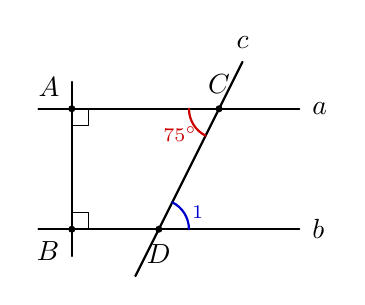
\begin{tikzpicture}[scale=0.85, >=stealth, line join=round, line cap=round]
  % Duong thang vuong goc AB
  \draw[thick] (0.8, 0.3) -- (0.8, 2.9);
  % Duong thang a di qua A
  \draw[thick] (0.3, 2.5) -- (4.2, 2.5) node[right=1pt] {$a$};
  % Duong thang b di qua B
  \draw[thick] (0.3, 0.7) -- (4.2, 0.7) node[right=1pt] {$b$};
  % Cat tuyen c di qua C va D (C(3.0, 2.5) va D(2.1, 0.7))
  \draw[thick] (3.35, 3.2) node[above=1pt] {$c$} -- (1.75, -0.0);
  
  % Giao diem A va B
  \fill (0.8, 2.5) circle (1.5pt) node[above left=1pt] {$A$};
  \fill (0.8, 0.7) circle (1.5pt) node[below left=1pt] {$B$};
  % Ky hieu vuong goc tai A va B
  \draw (0.8, 2.25) -- (1.05, 2.25) -- (1.05, 2.5);
  \draw (0.8, 0.95) -- (1.05, 0.95) -- (1.05, 0.7);
  
  % Giao diem C va D
  \fill (3.0, 2.5) circle (1.5pt) node[above=2pt] {$C$};
  \fill (2.1, 0.7) circle (1.5pt) node[below=2pt] {$D$};
  
  % Cung goc nhon ACD (huong tu 180 do ve 243.4 do)
  \draw[red!80!black, thick] (3.0, 2.5) ++(180:0.45) arc (180:243.4:0.45);
  \node[red!80!black, font=\scriptsize] at (2.42, 2.12) {$75^\circ$};
  
  % Cung goc D1 (so le trong voi ACD)
  \draw[blue!80!black, thick] (2.1, 0.7) ++(0:0.45) arc (0:63.4:0.45);
  \node[blue!80!black, font=\scriptsize] at (2.68, 0.95) {$1$};
\end{tikzpicture}
\end{minipage}\par
\vspace{0.5mm}
\noindent\textit{Bài giải:}\dongke{9}
\\ \hline
\end{tabularx}

\vspace{1.2mm}

\noindent
\begin{tabularx}{\linewidth}{|X|}
\hline
\vspace{0.5mm}
\begin{minipage}[t]{0.65\linewidth}
\vspace{0pt}
\textbf{Câu 14 (1,0 điểm).} Cho hình vẽ bên, biết hai đường thẳng $x$ và $y$ cùng vuông góc với đường thẳng $MN$ lần lượt tại $M$ và $N$. Đường thẳng $d$ cắt $x$ tại $P$ và cắt $y$ tại $Q$ sao cho $\widehat{MPQ} = 50^\circ$.\par\vspace{0.4mm}
\textbf{a) (0,5 điểm)} Chứng minh rằng đường thẳng $x$ song song với đường thẳng $y$ ($x \parallel y$).\par\vspace{0.4mm}
\textbf{b) (0,5 điểm)} Tính số đo góc $\widehat{NQP}$ và góc $\widehat{Q}_1$.
\end{minipage}\hfill
\begin{minipage}[t]{0.33\linewidth}
\vspace{0pt}\centering
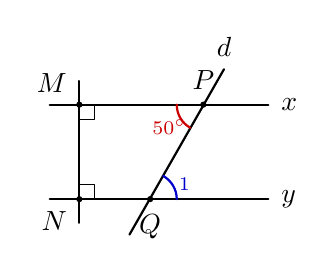
\begin{tikzpicture}[scale=0.75, >=stealth, line join=round, line cap=round]
  % Duong thang vuong goc MN
  \draw[thick] (0.8, 0.2) -- (0.8, 2.6);
  % Duong thang x di qua M
  \draw[thick] (0.3, 2.2) -- (4.0, 2.2) node[right=1pt] {$x$};
  % Duong thang y di qua N
  \draw[thick] (0.3, 0.6) -- (4.0, 0.6) node[right=1pt] {$y$};
  % Cat tuyen d di qua P va Q
  \draw[thick] (3.25, 2.8) node[above=1pt] {$d$} -- (1.65, -0.0);
  
  % Giao diem M va N
  \fill (0.8, 2.2) circle (1.5pt) node[above left=1pt] {$M$};
  \fill (0.8, 0.6) circle (1.5pt) node[below left=1pt] {$N$};
  % Ky hieu vuong goc tai M va N
  \draw (0.8, 1.95) -- (1.05, 1.95) -- (1.05, 2.2);
  \draw (0.8, 0.85) -- (1.05, 0.85) -- (1.05, 0.6);
  
  % Giao diem P va Q
  \fill (2.9, 2.2) circle (1.5pt) node[above=2pt] {$P$};
  \fill (2.0, 0.6) circle (1.5pt) node[below=2pt] {$Q$};
  
  % Cung goc nhon MPQ
  \draw[red!80!black, thick] (2.9, 2.2) ++(180:0.45) arc (180:240.6:0.45);
  \node[red!80!black, font=\scriptsize] at (2.32, 1.82) {$50^\circ$};
  
  % Cung goc Q1 (so le trong voi MPQ)
  \draw[blue!80!black, thick] (2.0, 0.6) ++(0:0.45) arc (0:60.6:0.45);
  \node[blue!80!black, font=\scriptsize] at (2.58, 0.85) {$1$};
\end{tikzpicture}
\end{minipage}\par
\vspace{0.4mm}
\noindent\textit{Bài giải:}\dongke{6}
\\ \hline
\end{tabularx}

\newpage

% =============================================================================
% ========================= TOÁN 7 - TUẦN 07 - BUỔI 02: MÃ ĐỀ 104 =============
% ========================= MẶT TRƯỚC (TRANG 1/2) ==============================
% =============================================================================

\noindent
\begin{tabularx}{\linewidth}{|X|c|}
\hline
\textbf{PHIẾU KIỂM TRA ĐỊNH KỲ TOÁN 7 - TUẦN 07 - BUỔI 02} & \textbf{Mã đề: 104 - Trang 1/2} \\
\hline
\end{tabularx}

\vspace{1.2mm}

\noindent
\begin{tabularx}{\linewidth}{|p{3.2cm}|X|}
\hline
\centering\textbf{ĐIỂM SỐ} & \centering\textbf{LỜI NHẬN XÉT CỦA THẦY CÔ} \tabularnewline
\hline
\rule{0pt}{1.8cm} & \tabularnewline
\hline
\end{tabularx}

\vspace{1.5mm}

\noindent\textbf{Câu 1 (0,25 điểm).} Số đối của số hữu tỉ $-\frac{11}{16}$ bằng bao nhiêu? \shortans{\frac{11}{16}}\par\vspace{0.5mm}
\noindent\textbf{Câu 2 (0,25 điểm).} Giá trị của biểu thức $\left(-\frac{2}{5}\right)^3$ bằng bao nhiêu? \shortans{-\frac{8}{125}}\par\vspace{0.5mm}
\noindent\textbf{Câu 3 (0,25 điểm).} Giá trị của căn bậc hai số học $\sqrt{\frac{25}{144}}$ bằng bao nhiêu? \shortans{\frac{5}{12}}\par\vspace{0.5mm}
\noindent\textbf{Câu 4 (0,25 điểm).} Tính giá trị của biểu thức $\lvert -9{,}3\rvert + \lvert -0{,}7\rvert$. \shortans{10}\par\vspace{0.5mm}
\noindent\textbf{Câu 5 (0,25 điểm).} Làm tròn số $41{,}736$ đến hàng phần trăm được kết quả là: \shortans{41{,}74}\par\vspace{0.5mm}
\noindent\textbf{Câu 6 (0,25 điểm).} Cho hai góc $\widehat{aOb}$ và $\widehat{bOc}$ kề bù, biết $\widehat{aOb}=70^\circ$. Số đo góc $\widehat{bOc}$ là: \shortans{110^\circ}\par\vspace{0.5mm}
\noindent\textbf{Câu 7 (0,25 điểm).} Tia $Oz$ là phân giác của góc $\widehat{xOy}$. Biết $\widehat{xOz}=55^\circ$, số đo $\widehat{xOy}$ là: \shortans{110^\circ}\par\vspace{0.5mm}
\noindent\textbf{Câu 8 (0,25 điểm).} Lập luận từ giả thiết để suy ra kết luận của một định lí gọi là gì? \shortans{\text{Chứng minh định lí}}\par\vspace{0.5mm}
\noindent\textbf{Câu 9 (0,25 điểm).} Hai đường thẳng phân biệt cùng vuông góc với một đường thẳng thứ ba thì chúng: \shortans{\text{song song}}\par\vspace{0.5mm}
\noindent\textbf{Câu 10 (0,25 điểm).} Quyển vở có giá $20\,000$ đ, được giảm giá $20\%$. Số tiền người mua phải trả là: \shortans{16\,000\text{ đ}}\par\vspace{0.5mm}
\vspace{0.6mm}

\noindent\textbf{Câu 11 (2,0 điểm). Thực hiện phép tính (hợp lý nếu có thể):}
\vspace{0.8mm}

\noindent
\begin{tabularx}{\linewidth}{|X|X|}
\hline
\oBaiTap[10]{a)}{$\frac{11}{18} + \left(-\frac{4}{5}\right) + \frac{7}{18}$} & 
\oBaiTap[10]{b)}{$\frac{14}{25} \cdot \left(-\frac{8}{13}\right) + \frac{14}{25} \cdot \left(-\frac{5}{13}\right)$} \\
\hline
\oBaiTap[10]{c)}{$\left(-\frac{2}{3}\right)^2 \cdot 18 - 1{,}5 \cdot 4$} & 
\oBaiTap[10]{d)}{$\sqrt{\frac{36}{25}} - \lvert -0{,}2\rvert + \sqrt{81}$} \\
\hline
\end{tabularx}

\newpage
% =============================================================================
% ========================= TOÁN 7 - TUẦN 07 - BUỔI 02: MÃ ĐỀ 104 =============
% ========================= MẶT SAU (TRANG 2/2) ================================
% =============================================================================

\noindent
\begin{tabularx}{\linewidth}{|X|c|}
\hline
\textbf{TOÁN 7 - TUẦN 07 - BUỔI 02} & \textbf{Mã đề: 104 - Trang 2/2} \\
\hline
\end{tabularx}

\vspace{1.2mm}

\noindent\textbf{Câu 12 (2,0 điểm). Tìm số hữu tỉ $x$, biết:}
\vspace{0.6mm}

\noindent
\begin{tabularx}{\linewidth}{|X|X|}
\hline
\oBaiTap[5]{a)}{$x + \frac{1}{6} = \frac{5}{12}$} & 
\oBaiTap[5]{b)}{$\frac{5}{6}x - \frac{1}{4} = \frac{7}{12}$} \\
\hline
\oBaiTap[5]{c)}{$\left(x + \frac{1}{2}\right)^2 = \frac{25}{4}$} & 
\oBaiTap[5]{d)}{$\lvert 3x + 1\rvert = 8$} \\
\hline
\end{tabularx}

\vspace{1.2mm}

\noindent
\begin{tabularx}{\linewidth}{|X|}
\hline
\vspace{0.5mm}
\begin{minipage}[t]{0.65\linewidth}
\vspace{0pt}
\textbf{Câu 13 (2,5 điểm).} Cho hình vẽ bên, biết hai đường thẳng $a$ và $b$ cùng vuông góc với đường thẳng $AB$ lần lượt tại $A$ và $B$. Đường thẳng $c$ cắt $a$ tại $C$ và cắt $b$ tại $D$ sao cho $\widehat{ACD} = 80^\circ$.\par\vspace{0.4mm}
\textbf{a) (1,25 điểm)} Chứng minh rằng đường thẳng $a$ song song với đường thẳng $b$ ($a \parallel b$).\par\vspace{0.4mm}
\textbf{b) (1,25 điểm)} Tính số đo góc $\widehat{BDC}$ và góc $\widehat{D}_1$.
\end{minipage}\hfill
\begin{minipage}[t]{0.33\linewidth}
\vspace{0pt}\centering
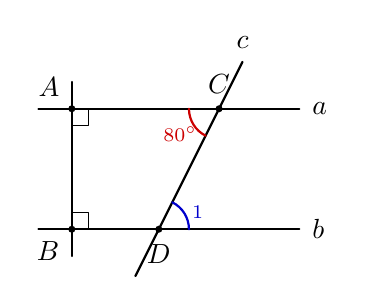
\begin{tikzpicture}[scale=0.85, >=stealth, line join=round, line cap=round]
  % Duong thang vuong goc AB
  \draw[thick] (0.8, 0.3) -- (0.8, 2.9);
  % Duong thang a di qua A
  \draw[thick] (0.3, 2.5) -- (4.2, 2.5) node[right=1pt] {$a$};
  % Duong thang b di qua B
  \draw[thick] (0.3, 0.7) -- (4.2, 0.7) node[right=1pt] {$b$};
  % Cat tuyen c di qua C va D (C(3.0, 2.5) va D(2.1, 0.7))
  \draw[thick] (3.35, 3.2) node[above=1pt] {$c$} -- (1.75, -0.0);
  
  % Giao diem A va B
  \fill (0.8, 2.5) circle (1.5pt) node[above left=1pt] {$A$};
  \fill (0.8, 0.7) circle (1.5pt) node[below left=1pt] {$B$};
  % Ky hieu vuong goc tai A va B
  \draw (0.8, 2.25) -- (1.05, 2.25) -- (1.05, 2.5);
  \draw (0.8, 0.95) -- (1.05, 0.95) -- (1.05, 0.7);
  
  % Giao diem C va D
  \fill (3.0, 2.5) circle (1.5pt) node[above=2pt] {$C$};
  \fill (2.1, 0.7) circle (1.5pt) node[below=2pt] {$D$};
  
  % Cung goc nhon ACD (huong tu 180 do ve 243.4 do)
  \draw[red!80!black, thick] (3.0, 2.5) ++(180:0.45) arc (180:243.4:0.45);
  \node[red!80!black, font=\scriptsize] at (2.42, 2.12) {$80^\circ$};
  
  % Cung goc D1 (so le trong voi ACD)
  \draw[blue!80!black, thick] (2.1, 0.7) ++(0:0.45) arc (0:63.4:0.45);
  \node[blue!80!black, font=\scriptsize] at (2.68, 0.95) {$1$};
\end{tikzpicture}
\end{minipage}\par
\vspace{0.5mm}
\noindent\textit{Bài giải:}\dongke{9}
\\ \hline
\end{tabularx}

\vspace{1.2mm}

\noindent
\begin{tabularx}{\linewidth}{|X|}
\hline
\vspace{0.5mm}
\begin{minipage}[t]{0.65\linewidth}
\vspace{0pt}
\textbf{Câu 14 (1,0 điểm).} Cho hình vẽ bên, biết hai đường thẳng $x$ và $y$ cùng vuông góc với đường thẳng $MN$ lần lượt tại $M$ và $N$. Đường thẳng $d$ cắt $x$ tại $P$ và cắt $y$ tại $Q$ sao cho $\widehat{MPQ} = 65^\circ$.\par\vspace{0.4mm}
\textbf{a) (0,5 điểm)} Chứng minh rằng đường thẳng $x$ song song với đường thẳng $y$ ($x \parallel y$).\par\vspace{0.4mm}
\textbf{b) (0,5 điểm)} Tính số đo góc $\widehat{NQP}$ và góc $\widehat{Q}_1$.
\end{minipage}\hfill
\begin{minipage}[t]{0.33\linewidth}
\vspace{0pt}\centering
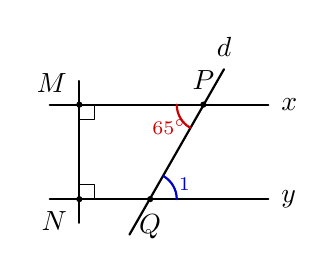
\begin{tikzpicture}[scale=0.75, >=stealth, line join=round, line cap=round]
  % Duong thang vuong goc MN
  \draw[thick] (0.8, 0.2) -- (0.8, 2.6);
  % Duong thang x di qua M
  \draw[thick] (0.3, 2.2) -- (4.0, 2.2) node[right=1pt] {$x$};
  % Duong thang y di qua N
  \draw[thick] (0.3, 0.6) -- (4.0, 0.6) node[right=1pt] {$y$};
  % Cat tuyen d di qua P va Q
  \draw[thick] (3.25, 2.8) node[above=1pt] {$d$} -- (1.65, -0.0);
  
  % Giao diem M va N
  \fill (0.8, 2.2) circle (1.5pt) node[above left=1pt] {$M$};
  \fill (0.8, 0.6) circle (1.5pt) node[below left=1pt] {$N$};
  % Ky hieu vuong goc tai M va N
  \draw (0.8, 1.95) -- (1.05, 1.95) -- (1.05, 2.2);
  \draw (0.8, 0.85) -- (1.05, 0.85) -- (1.05, 0.6);
  
  % Giao diem P va Q
  \fill (2.9, 2.2) circle (1.5pt) node[above=2pt] {$P$};
  \fill (2.0, 0.6) circle (1.5pt) node[below=2pt] {$Q$};
  
  % Cung goc nhon MPQ
  \draw[red!80!black, thick] (2.9, 2.2) ++(180:0.45) arc (180:240.6:0.45);
  \node[red!80!black, font=\scriptsize] at (2.32, 1.82) {$65^\circ$};
  
  % Cung goc Q1 (so le trong voi MPQ)
  \draw[blue!80!black, thick] (2.0, 0.6) ++(0:0.45) arc (0:60.6:0.45);
  \node[blue!80!black, font=\scriptsize] at (2.58, 0.85) {$1$};
\end{tikzpicture}
\end{minipage}\par
\vspace{0.4mm}
\noindent\textit{Bài giải:}\dongke{6}
\\ \hline
\end{tabularx}

\newpage

\end{document}
